%%*************************************************************************
%%
%% Optimalization of the Assembly Line Manufacturing Processes
%% 
%% 2012/03/05
%% by Peter Boraros
%% See http://www.pborky.sk/contact for current contact information.
%%
%%*************************************************************************
%%
%% Legal Notice:
%%
%% This code is offered as-is without any warranty either expressed or
%% implied; without even the implied warranty of MERCHANTABILITY or
%% FITNESS FOR A PARTICULAR PURPOSE! 
%% User assumes all risk.
%%
%% This work by Peter Boraros is licensed under a 
%% Creative Commons Attribution-NonCommercial-ShareAlike 3.0 Unported License.
%% http://creativecommons.org/licenses/by-nc-sa/3.0/
%%
%%*************************************************************************

\documentclass[a4paper,journal,twocolumn]{IEEEtran}

\usepackage{cite}
% \usepackage[nocompress]{cite}
\usepackage{ifpdf}

\ifpdf
\usepackage[pdftex]{graphicx}
\graphicspath{{./img/}}
\DeclareGraphicsExtensions{.pdf}
\else
\usepackage[dvips]{graphicx}
\graphicspath{{./img/}}
\DeclareGraphicsExtensions{.eps}
\fi

\usepackage[margin=30mm]{geometry}

\usepackage{graphviz}

\usepackage[cmex10]{amsmath}
\usepackage{amsfonts}
\usepackage{amssymb}
\interdisplaylinepenalty=2500

\usepackage{algorithmic}

\usepackage{array}

\usepackage{mdwmath}
\usepackage{mdwtab}

\usepackage{eqparbox}

\usepackage[hang,small,center,bf]{caption}
% \usepackage[tight,normalsize,sf,SF]{subfigure}
%\usepackage[tight,footnotesize]{subfigure}
\usepackage{subfig}
% \usepackage[caption=false,font=normalsize,labelfont=sf,textfont=sf]{subfig}
% \usepackage[caption=false,font=footnotesize]{subfig}

\usepackage[utf8x]{inputenc}
%\usepackage[czech]{babel}
%\usepackage[T1]{fontenc}


%\usepackage{url}
\usepackage[colorlinks=true,urlcolor=blue]{hyperref}
\usepackage{fixltx2e}
\usepackage{stfloats}
\usepackage{ucs}
\usepackage{multirow}

% correct bad hyphenation here
\hyphenation{op-tical net-works semi-conduc-tor}

\renewcommand{\labelitemi}{$\bullet$}
\renewcommand{\labelitemii}{$\circ$}
\renewcommand{\labelitemiii}{$\ast$}


%\setlength{\textheight}{290mm}

\begin{document}

\title{Optimalization of the Manufacturing Processes on the Assembly Line}
\date{March 05, 2012}
\author{Peter~Boráros %
\thanks{{Peter Boráros}, Czech Technical University in Prague,
see~\href{http://www.pborky.sk/contact}{\scriptsize{\texttt{http://www.pborky.sk/contact}}} for a contact infomation}}%

% The paper headers
%\markboth{Peter Boráros, Czech technical university, Faculty of Electrical Engineering, Prague, Czech Republic}{}

%\IEEEcompsoctitleabstractindextext{%
%\begin{abstract}

%\end{abstract}}

\maketitle
\IEEEdisplaynotcompsoctitleabstractindextext
\IEEEpeerreviewmaketitle

\section{The problem}\label{ass}
The task is to design and implement scheduling algorithm for assembly manufacturing line group.
Group is described by directed acyclic graph with one output and several input nodes (see
~\emph{fig.~\ref{fig:graph}}). Input nodes repesent input buffer of the material and output node represents
output buffer of the product. Inner nodes represent assembly machines or control points.
One or more machines or control points are handled by operator. Operator must be qualified for 
position where he works. Operator`s skills can affect the productivity.

Manufacturing line group can produce several models of the product based on setup of the 
machines. Modification to the setup takes defined time and consumes resources of the
technical support group (technicians and engineers).

Given is material availability, presence of the operator and technical staff, the production plan,
the production rate for particular machines, the probability of the defective material in 
particular input buffer and the probability of the defect in process of production for particular
checkpoint.

Output of algorithm is time schedule of the production setups for particular machines as the 
placement of the operator and technical staff (it must be capable to handle with lack of staff).
Algorithm maximizes the production quantity. The constraints are shipment schedule to
the customer and estimate of material availability. Time is discrete and time step is given.


The problem can be categorised as job-shop scheduling problem. The tasks are production orders (instructions for the operators).
The production order (task) depicts an ammount produced model (or duration of the production) and the description of the model
at the particular time span.
Jobs are sets of tasks for particular resource.
The resources are prodution machines and material or subassemblies used by machine.
Availability of the resources is limited by setup or maintence process or by production of the subassemblies
on the upstream assembly line or by shipment of the material from the suppliers.
%Limitations of the availability can be caused by the change of particular task for another taks.

\section{Related works}
Most common methodology in job-shop scheduling is material resource planning (MRP). As the MRP is the planning tool it
is not designed for the detailed scheduling. In practice the scheduling is performed by experienced shop-floor
personel with pencil. 
For solving immediate problems, such as sequencing, dispatching rules are often used. 
There have been implemented dispatching rules and heuristics  based on  due dates, criticalicity of the operations, 
processing times and resource utilization. 
Such heuristics and rules were used also in artificial intelligence approaches.\cite{Hoi}

Other methods have been developed based on optimalization methodologies such as \emph{dynamic programming} or 
\emph{branch-and-bound} method.
These methods require at least partial enumeration of possible sequences and thus computational complexity grows exponentially
as the problem size increases. Additionally the schedule is no longer optimal after minor changes in tasks or addition of the 
new tasks or breakdown of the machine.\cite{Hoi}

\emph{Langragian relaxation} method has been developped to solve scheduling problem. 
Method is used to decompose the problem into set of smaller subproblems, 
providing tight lower bound on optimal cost.\cite{Hoi}
The langragian problem can be used to probide bounds in branch-and-bounds algorithm.
This approach lead to increase performance for several problems such as routing problem, scheduling and set covering.\cite{Fis}

Because of NP-completeness of the mixed integer model the methods based on solving integer programs can only be used for 
small problems. Therefore, other representations and algorithms are widely used instead of linear programming. For example
\emph{stochastic search} methods are used to perturbate search space usign stochastic operators and search space cut process.
Common are methods based on genetic algorithm as described in \cite{Sed} or \cite{Uni}. We will describe method based 
on genetic algorith usable to solve job-shop scheduling problem.

\section{Problem solution}
\subsection{Linear programming}
Let us define variables used for integer programming problem formulation:
\begin{itemize}
	\item $\mathcal{J}$ -- set of jobs,
	\item $\mathcal{O}$ -- set of all operations,
	\item $\mathcal{M}$ -- set of all resources,
	\item $\left(i,j\right) \in \mathcal{O}$ -- $j$-th operation of job $j \in \mathcal{J}$,
	\item $m_{o}\in\mathcal{M}$ -- resource where operation $o\in\mathcal{O}$ is to be executed,
	\item $b_{o}$ -- starting time of operation $o\in\mathcal{O}$,
	\item $p_{o}$ --  processing time of operation $o\in\mathcal{O}$ ($p_{o}\ge 0$),
	\item $\prec_o : \mathcal{O} \rightarrow \mathcal{O}$ -- precedence relation between two operations of same job (it is not transitive),
	\item $r_{o}$ -- release time of operation $o\in\mathcal{O}$ ($r_{o} \ge 0$),
	\item $s_{o_1,o_2}$ -- setup time before operation $o_2$ after operation $o_1$
	has been processed ($o_1,o_2\in\mathcal{O}$),
	\item $\tilde{d_i}$ -- deadline of job $i\in\mathcal{J}$ ($\tilde{d_i}> 0$),
	\item $\max_{o\in\mathcal{O}} (b_o+p_o)$ -- makespan (completion time of the last job).
\end{itemize}

We will use term job to denote production order for particular model. Deadline of job $\tilde{d_j}$ is defined by same production order.
Each job $j\in\mathcal{J}$ consist of a set of operations $o\in\mathcal{O}$ each of which needs 
to be processed during an uninterupted time period of a given length $p_o$ on a given resource $m_o$.
Precedence relation $\prec_o$ denotes technological link-up that is graphically represented by graph 
(e.g.~\emph{fig.~\ref{fig:graph}}) and following formula holds 
$\forall o_1=(i,j)\in\mathcal{O};o_2=(k,l)\in\mathcal{O}: o_1\prec_oo_2 \implies i=k $ -- so the precedence is defined only between
operations of the same job.
Each resource $m\in\mathcal{M}$ can process at most one operation at a time.
Release time of operation $r_o$ is time when operation is available for scheduling. It is deterined by
material presence at input buffers and by operator presence at defined position.

Let us denote makespan $C_{max} = \max_{o\in\mathcal{O}}\left(b_o + p_o\right)$ and 
delay between operations $o$, $p$:  $D_o = \left(b_o + p_o +s_{o,p}-b_p\right), \mathsf{iff}\; \exists p: o \prec_o p\; \mathsf{otherwise}\;D_o= 0$.
The problem of optimal job shop scheduling is to find starting time $b_o$ of each operation $o\in\mathcal{O}$ such that
\begin{equation}\label{eq:subject}
	 \sum_{o\in\mathcal{O}}D_o + C_{max}
\end{equation}
is minimized subject to
\begin{equation} \label{eq:lowboundzero}
	\forall o\in\mathcal{O}: b_o \ge 0 
\end{equation}
\begin{equation}\label{eq:lowbound}
	\forall o\in\mathcal{O}: b_o \ge r_o
\end{equation}
\begin{equation}\label{eq:upperbound}
	\forall j \in \mathcal{J}: \forall o=(j,k)\in\mathcal{O}: b_o\le \tilde{d_j}-p_o
\end{equation}
\begin{equation}\label{eq:precconstraints}
	\forall o,p \in\mathcal{O}, o\prec_o p:b_p \ge b_o+p_o+s_{o,p}
\end{equation}
\begin{align}\label{eq:capconstraints}
	& \forall o,p\in\mathcal{O},o=(i,k),p=(j,l),o\neq p, \\
	& \{i,j\}\subseteq\mathcal{J}, m_o=m_p\in \mathcal{M}: \nonumber \\
	& (b_o \ge b_p+p_p+s_{p,o}) \vee  (b_p \ge b_o+p_o+s_{o,p})  \nonumber 
\end{align}

In (\ref{eq:subject}) we can use more relaxed precedence operator to denote $D$ such that it will penalize 
only delays between operations on one machine group and we will denote this operator ($\prec_g$). The effect 
of this relaxation more flexibility in operation schedule.

As inequalities (\ref{eq:lowbound}) gives tighter \emph{lower bound} than (\ref{eq:lowboundzero}) we can ommit
(\ref{eq:lowboundzero}).
Conditions (\ref{eq:upperbound}) express \emph{upper bound}. Conditions (\ref{eq:precconstraints}) express
\emph{precedence constraints} and (\ref{eq:capconstraints}) express resource \emph{capacity constraints}
i.e. each resource can process one operation at a time.

Precedence constraints (\ref{eq:precconstraints}) consists of varying number of inequalities depending on 
precedence relation~($\prec_o$). Capacity constraints (\ref{eq:capconstraints}) cannot be used directly 
because disjunction operator ($\vee$) must be eliminated first.

Let us introduce new variable $x_{o,p}\in\left\{0,1\right\}$ where $o,p\in\mathcal{O}$. 
Let us define $x_{o,p} = 1 $ iff $m_o = m_p $ and operation $o$ precedes $p$.
The precedence constraints (\ref{eq:precconstraints}) can be replaced with following equations
(note that $p_o+s_{o,p} + \tilde{d_i}$ is constant):
\begin{align}
	& \forall o,p\in\mathcal{O},o=(i,k),p=(j,l),o\neq p, \nonumber \\
	& \{i,j\}\subseteq\mathcal{J}, m_o=m_p\in \mathcal{M}: \nonumber \\
	& b_p \ge b_o + x_{o,p}(p_o+s_{o,p} + \tilde{d_i}) - \tilde{d_i}\\
	&  x_{o,p}+x_{p,o} = 1
\end{align}

So job-shop scheduling problem can be reformulated as problem of finding $b_o$ of each operation
$o\in\mathcal{O}$ such that
\begin{equation}\label{eq:subject2}
	 \sum_{o\in\mathcal{O}}D_o + C_{max}
\end{equation}
is minimized subject to
\begin{equation}\label{eq:lowbound2}
	\forall o\in\mathcal{O}: b_o \ge r_o
\end{equation}
\begin{equation}\label{eq:upperbound2}
	\forall j \in \mathcal{J}: \forall o=(j,k)\in\mathcal{O}: b_o\le \tilde{d_j}-p_o
\end{equation}
\begin{equation}\label{eq:precconstraints2}
	\forall o,p \in\mathcal{O}, o\prec_o p:b_p \ge b_o+p_o+s_{o,p}
\end{equation}
\begin{equation}\label{eq:x}
\forall o,p\in\mathcal{O},o\neq p: x_{o,p}+x_{p,o} = 1
\end{equation}
\begin{align}\label{eq:capacity2}
	& \forall o,p\in\mathcal{O},o=(i,k),p=(j,l),o\neq p, \\
	& \{i,j\}\subseteq\mathcal{J}, m_o=m_p\in \mathcal{M}: \nonumber \\
	& b_p \ge b_o + x_{o,p}(p_o+s_{o,p} + \tilde{d_i}) - \tilde{d_i}\nonumber
\end{align}

We can sovle the problem (\ref{eq:subject2}) - (\ref{eq:capacity2}) by relaxing integrality constraints
and using linear programing approach. Unfortunately it is hard to find solution to this problem.

We now adopt \emph{Langragian relaxation approach}. 
Precedence constraints (\ref{eq:precconstraints2}) can be relaxed using the nonnegative Langrange multipliers $\lambda_{o,p}$
and the capacity constaints (\ref{eq:capacity2}) can be relaxed using the nonnegative Langrange multipliers $\pi_{o,p}$.
Let us denote $a_{o,p} = b_o + p_o + s_{o,p}$ and $d_{o,p} = p_o + s_{o,p}$
So the Langragian problem (LR) formulation is 
\begin{align}
	& Z_{LR}\left(b,x\right)=\sum_{o\in\mathcal{O}}D_o + C_{max} + \sum_{o,p\in\mathcal{O}}\lambda_o\left(b_p-a_{o,p}\right) + \nonumber \\
	& +\sum_{o,p\in\mathcal{O}}\pi_{o,p}\left(b_p-b_o-x_{o,p}(d_{o,p}+\tilde{d}_i)+\tilde{d}_i\right) 
\end{align}
is minimized subject to (\ref{eq:upperbound2}), (\ref{eq:lowbound2}) and (\ref{eq:x}).

In order to solve the problem LR we must find values of multipliers $\lambda$ and $\pi$. This can be achieved by
solving dual problem (D) such that 
\begin{align}
	& Z_{LR}\left(\pi,\lambda\right)\nonumber
\end{align}
is maximized subject to (\ref{eq:upperbound2}), (\ref{eq:lowbound2}) and (\ref{eq:x}).

\subsection{Stochastic search}
In this section we will describe genetic algorithm developed to solve job-shop scheduling problem.
The genetic algorithms are well known we briefly concentrate on problem specific details.

Let us express chromosome as set of permutatinons of jobs where each element in set is gene and is related to particular resource.
Crossover operator would be two-point crossover, where middle part of one chromosome is exchanged.
For mutation operator we can adopt exchange mutation where it changes randomly selected gene (permutation). In \cite{Sed} author suggest
shift mutation where it removes value at one position and puts in to another position.

Size of population would be 50. Suggested selection algorithm would be stochastic universal sampling, where defined number of individuals
are selected with probability proportional to their fitness walue in process called roullete wheel selection.

Optimalisation objective is determined by (\ref{eq:subject2}), so the fitness value is derived from it, but in additon
individual which violates constraints (\ref{eq:lowbound2}), (\ref{eq:upperbound2}) is given fitness value of zero
and thus cannot pass selection process. This individual would be allowed to undergo mutation process.

The permutation of jobs at each resource determines starting time of particular operation 
and the gap between operations are as small as possible respecting capacity constraint (\ref{eq:capconstraints}).

\section{Experiments}
In this section we will present solution to linear programming problems, that were described in past section.
For this we will use modeling language PuLP that is Python-based environment with interface to several solver engines like CPLEX, GLPK, DIP, etc.

The simple program written in python programming language implements instance of job-shop graphically represented on \emph{fig. \ref{fig:graph}}.
There is fixed number of operations per job determined by vertices of graph.
Problem definition can be found in procedure \texttt{problem()}  in file \texttt{jobshop.py}. 
The procedure outputs intermediate representation 
and CPLEX representation is written to file \texttt{test.cpxlp}.

The program outputs an operation schedule in tabular form and also the gantt graph that is graphical representation of the schedule and can be seen on
\emph{fig. \ref{fig:gantt}}. 



\begin{thebibliography}{1}

\bibitem{Hoi} \textsc{D.J. Hoitomt}, \textsc{P.B. Luh}, and \textsc{K.R. Pattipati}, \emph{Practical Approach to Job-Shop Scheduling
Problems}, 1-13, IEEE Trans Rob Autom, Feb, 9(1), 1993.

\bibitem{Fis} \textsc{Marshall L. Fisher}, \emph{The langragian relaxation method for solving linear integer problems}, 1-17, 
Management Science, Vol. 27, No. 1, 1981.

\bibitem{Sed} \textsc{Miloš Šeda}, \emph{Mathematical Models of Flow Shop and Job Shop Scheduling Problem}, 122-127, World Academy of Science, Engineering and Technology 31, 2007.

\bibitem{Uni} \textsc{Takeshi Yamada, Ryohei Nakano}, \emph{Genetic Algorithms for Job-Shop  Scheduling Problems}, 67–81, Proceedings of Modern Heuristic for Decision Support, 1997.

\bibitem{Dip} \textsc{Michael O’Sullivan, Qi-Shan Lim, Cameron Walker, Iain Dunning, Stuart Mitchell}, \emph{Dippy – a simplified interface for advanced mixed-integer programming}, Report, University of Auckland, Faculty of Engineering, no. 685, 2012.

%\bibitem{} \textsc{}, \emph{}, , .

\end{thebibliography}

\clearpage
\onecolumn
\appendix

\begin{figure}[h]%
  \centering
  \digraph[width=150mm]{MyGraph}{
    rankdir=LR;
	subgraph cluster_0 {
		node [style=filled];
		a0 [shape=square];
		a2 [shape=square];
		a1 [shape=diamond];
		a3 [shape=diamond];
		a0 -> a1 -> a4;
		a2 -> a3 -> a4;
		label = "subassembly";
		color=lightblue;
		style=filled;
	} 
	subgraph cluster_1 {
		node [style=filled];
		b0 [shape=square];
		b1 [shape=diamond];
		b0 -> b1 -> b2 -> b4;
		label = "PCB";
		color=lightblue;
		style=filled;
	}  
	subgraph cluster_2 {
		node [style=filled];
		c0 [shape=square];
		c1 [shape=diamond];
		c0 -> c1 -> c2;
		label = "heatsink";
		color=lightblue;
		style=filled;
	}
	subgraph cluster_3 {
		node [style=filled];
		d0 [shape=square];
		d1 [shape=diamond];
		d2 [shape=diamond];
		d3 [shape=diamond];
		d0 -> d1 -> d4;
		d2 -> d4;
		d3 -> d4;
		label = "assembly";
		color=lightblue;
		style=filled;
	}
	subgraph cluster_4 {
  		node [style=filled];
  		f1 [shape=diamond];
		f1 -> f2;
		label = "packing";
		color=lightblue;
		style=filled;
	}
	b4 -> c2 -> d3;
	a4 -> d2;
	d4 -> f1;
  }
  \caption{Example of production line group. Blue clusters represent particular assembly lines
  and operator position. 
  The input buffers are nodes of square shape and checkpoints are of diamond shape.}
  \label{fig:graph}
\end{figure}

\begin{figure}[h]%
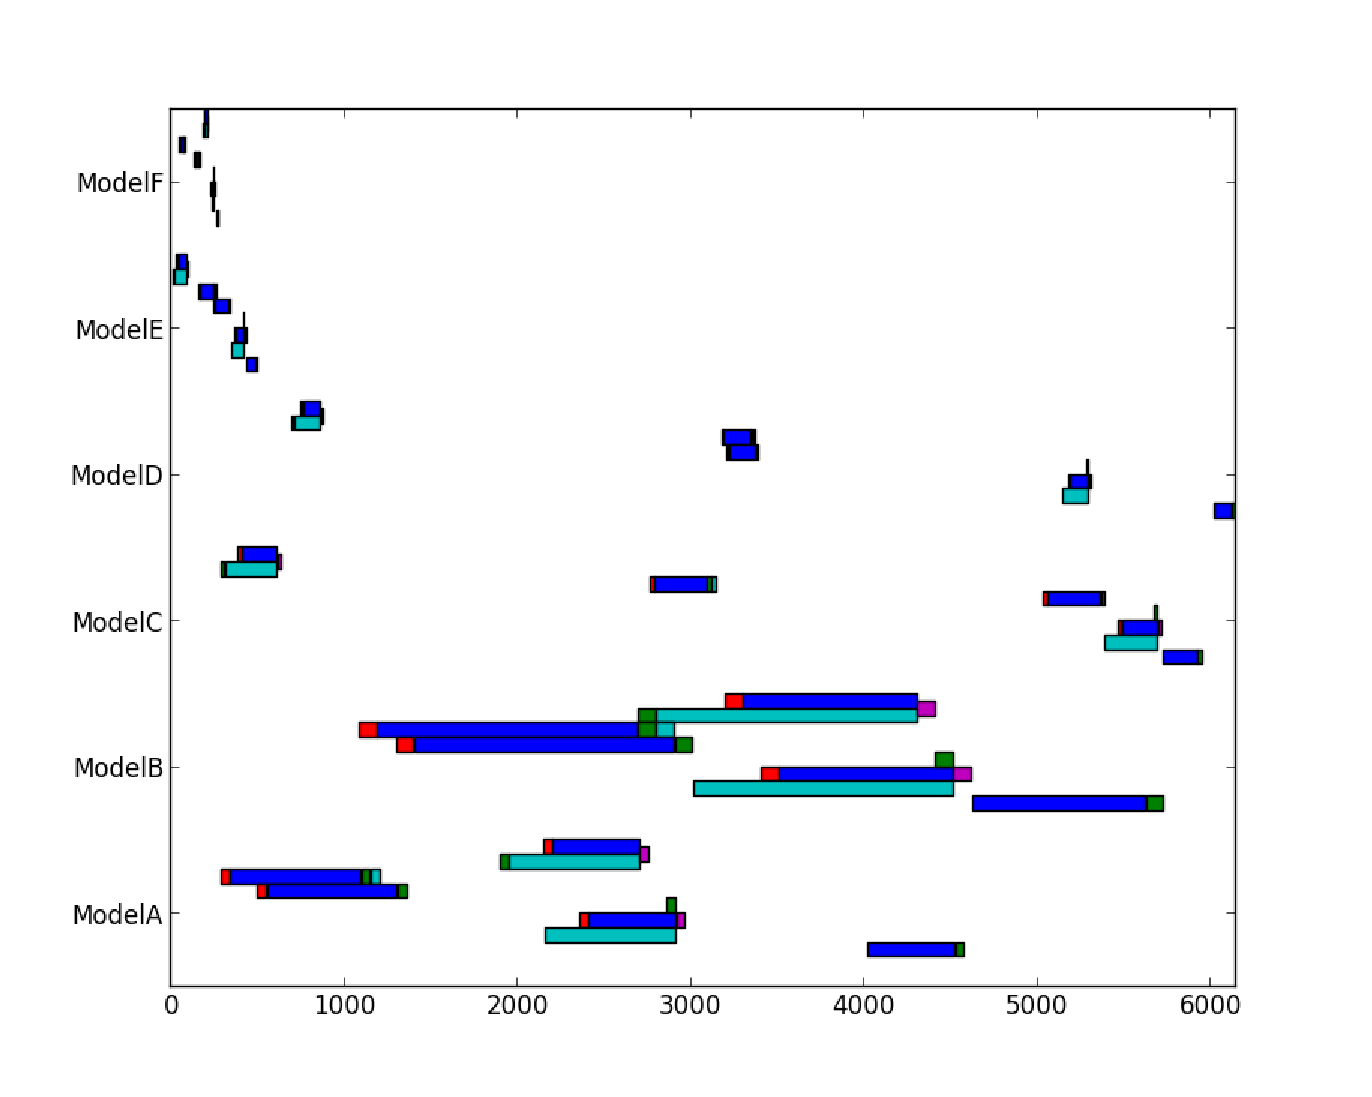
\includegraphics[width=150mm]{gantt}
  \centering  \caption{Gantt chart expressing schedule of five models (jobs) given  technology graph on fig. \ref{fig:graph} }
  \label{fig:gantt}
\end{figure}
% that's all folks
\end{document}
